\section{Component Architecture} \label{sc:component_architecture}
With the criteria defined, the overall component architecture of the system can be designed. Below is a diagram of the different components of the system, followed by a description.

\begin{figure}[H]
    \centering
    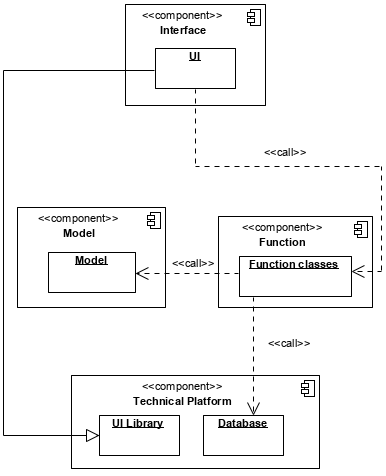
\includegraphics[width=0.6\textwidth]{figures/ComponentDiagrams/ComponentDesignOverview.png}
    \caption{An overview of the overall component design}
    \label{fig:OverviewOfComponentDesign}
\end{figure}
As seen in \autoref{fig:OverviewOfComponentDesign} the architecture of the system closely resembles the "Generic Architecture Pattern" described in \citep[p 198]{OOAD}.
\par
At the bottom is the technical platform, which contains a UI Library and a database. In the center to the left is the model component, which stores the model of the problem domain. To the right of this is the function component, which contains classes, which implements most of the functionality of the system. At the top of the diagram is the interface component, which only contains the UI, as the system will only communicate with the database and the users.
\par
The classes in the model can be utilized and manipulated by the function classes, which is the reason for the call connection between the two subcomponents. These are triggered by interactions between the users and the system in the UI, which is the cause of the call connection between the UI and the function classes. The UI is based off of the UI Library, which means the UI is a specialization of the UI Library. Lastly, the function classes will handle the communication with the database and is therefore connected to it by a call connection.
\par
In the following sections, the different components will be examined and described in further detail.